\documentclass[12pt]{article}

\usepackage[numbers,sort]{natbib}
\usepackage{amsfonts, amsmath}
\usepackage{graphicx}
% Libertine (optional): \texttt{tlmgr install libertine} — then swap in \texttt{\textbackslash usepackage\{libertine\}}
\usepackage{lmodern}
% \usepackage{fullpage} % e.g. tlmgr install preprint — margins are handled by geometry below
\usepackage{xcolor}
\usepackage{hyperref}
% cleveref (optional): tlmgr install cleveref
\usepackage{float}
\hypersetup{
    colorlinks = true,
    linkcolor = blue,
    urlcolor  = blue,
    citecolor = blue,
    anchorcolor = blue}
\newcommand{\todo}[1]{\textcolor{red}{[TODO: #1]}}
\urlstyle{same}
% caption / subcaption / siunitx: tlmgr install caption subcaption siunitx
\usepackage{booktabs}
\graphicspath{{figures/}}
\usepackage[a4paper,margin=1in]{geometry}
% setspace / parskip: tlmgr install setspace parskip
% listings: tlmgr install listings — then restore lstset block from report history if needed

%%%%%%%%%%%%%%%%%%%%%%%%%%%%%%%%%%%%%%%%%%%%%%%%%%%%%%%%%%%%%%%%%%%%%%%%%%%%%%%%%%%%%%
% Document
%%%%%%%%%%%%%%%%%%%%%%%%%%%%%%%%%%%%%%%%%%%%%%%%%%%%%%%%%%%%%%%%%%%%%%%%%%%%%%%%%%%%%%
\begin{document}

%%%%%%%%%%%%%%%%%%%%%%%%%%%%%%%%%%%%%%%%%%%%%%%%%%%%%%%%%%%%%%%%%%%%%%%%%%%%%%%%%%%%%%
% Cover / Title page
%%%%%%%%%%%%%%%%%%%%%%%%%%%%%%%%%%%%%%%%%%%%%%%%%%%%%%%%%%%%%%%%%%%%%%%%%%%%%%%%%%%%%%
\begin{titlepage}
    \centering

    \vspace*{1.0cm}
    
\includegraphics[width=0.4\textwidth]{nus_logo.jpg}

    \vspace{1.0cm}

    {\LARGE \textbf{Portfolio Risk Analyst Chatbot: \\[0.3cm]
    Quantitative Metrics, Retrieval-Augmented Guidance, \\[0.3cm]
    and Conversational Orchestration} \par}

    \vspace{1cm}

    {\large DSA4265 — Group 5 \par}
    \vspace{0.3cm}
    {\large \today \par}

    \vspace{1.0cm}

    \renewcommand{\arraystretch}{1.5}
    \begin{tabular}{|p{4.5cm}|p{3.5cm}|p{5cm}|}
        \hline
        \textbf{Name} & \textbf{Matric Number} & \textbf{Email} \\ \hline
        Liu Jingyan & A0258209Y & e0969181@u.nus.edu \\ \hline
        % Add your name and matric number here !
    \end{tabular}

    \vspace{0.5cm}

    \begin{minipage}{0.9\textwidth}
\small
\begin{center}
\textbf{Abstract}
\end{center}

Risk indicators shown in consumer applications are frequently opaque with respect to the portfolio weights to which they pertain, whilst unconstrained dialogue with large language models can yield numerically specific yet unsubstantiated statements drawn from parametric memory. This report describes a Streamlit-based conversational system that mitigates these issues by coupling user-supplied holdings to a reproducible analytics pipeline. Validated ticker--weight pairs drive a single download of split- and dividend-adjusted closing prices via Yahoo Finance (\texttt{yfinance}); consistent simple-return series underpin annualised volatility, a historical one-day loss quantile used as a VaR-style descriptor, maximum drawdown, a Sharpe-style ratio with the risk-free rate fixed at zero, mean pairwise correlation, and a Herfindahl concentration measure. User utterances are classified with Google Gemini into task types (holistic review, named statistics, definitional queries, and related categories); a deterministic orchestration layer then invokes quantitative computation, hybrid retrieval over local knowledge corpora (BM25 plus dense vectors in Chroma), or both, and formats the user-visible reply as Markdown without a separate generative rewriting stage in the reference interface. The architecture modularises analytics and retrieval to admit further risk measures or forecasting components; findings are contingent on vendor data quality and reporting delay, and the software is offered for research and pedagogical use only, not as regulated investment advice.

\end{minipage}

    \vfill
\end{titlepage}

\tableofcontents
\newpage

%%%%%%%%%%%%%%%%%%%%%%%%%%%%%%%%%%%%%%%%%%%%%%%%%%%%%%%%%%%%%%%%%%%%%%%%%%%%%%%%%%%%%%
% Main body (outline — expand in \texttt{sections/})
%%%%%%%%%%%%%%%%%%%%%%%%%%%%%%%%%%%%%%%%%%%%%%%%%%%%%%%%%%%%%%%%%%%%%%%%%%%%%%%%%%%%%%

\section{Introduction}
\label{sec:introduction}

\subsection{Motivation and problem statement}
Portfolio risk is inherently multidimensional: volatility, tail behaviour, co-movement among holdings, and weight concentration capture distinct facets of exposure, and user information needs vary accordingly. At the same time, interactive assistants based on large language models (LLMs) do not, by default, observe an end-user's asset allocation; numerical summaries produced without an explicit data channel therefore cannot be guaranteed to correspond to any stated portfolio.

A second concern is \emph{provenance}. Even high-quality natural-language explanations of financial concepts may be difficult to audit when they are generated solely from model weights rather than from retrievable evidence aligned to the question and, where relevant, to the user's positions.

\subsection{Objectives and scope}
The objective of the present work is a conversational interface through which, subject to prior validation of the portfolio specification, a user may obtain (i) an aggregated risk summary, (ii) values for implemented scalar risk statistics, (iii) definitional or contextual material on finance terminology, and (iv) short follow-up clarification anchored in the preceding system response. ``What-if'' and rebalancing-oriented questions are treated within the same analytical family as broad risk-review requests; the implementation records whether the allocation has changed relative to earlier session state.

The scope is instructional and prototypical. Live order execution, personalised advice governed by securities regulation, tax treatment, and production-grade risk reporting are excluded. Prices are taken as end-of-day vendor quotes adequate for coursework and proof-of-concept use, not as tick-level or certified reference data.

\subsection{Contributions}
The work is primarily engineering-centred; its contributions are architectural and empirical rather than theoretical:
\begin{itemize}
    \item A Streamlit application with structured portfolio capture, validation logic for tickers and weights, and session-persistent chat transcriptions via Streamlit session state.
    \item A unified data-access layer for adjusted closing prices, optionally augmented with a broad equity market proxy (SPY) on a common trading calendar, together with centralised return construction interfaces (simple and logarithmic) to standardise preprocessing contracts across analytical and prospective machine-learning components.
    \item A baseline quantitative module operating on historical daily returns, yielding annualised volatility, a historical one-day quantile usable as a rudimentary value-at-risk figure, a zero risk-free Sharpe-style ratio, maximum drawdown on the cumulative return path, average pairwise correlation among constituents, and a Herfindahl index of weights; these inputs map to a rule-based composite score and categorical risk band for narrative presentation.
    \item Structured intent inference (Google Gemini) coupled to explicit routing code that invokes the metric pipeline, attaches optional retrieval results, or surfaces recent assistant output for follow-up turns.
    \item A retrieval-augmented generation (RAG) subsystem comprising multiple curated corpora (including conceptual and strategy-oriented material), intent-conditioned source selection, hybrid lexical and dense-vector retrieval in Chroma, and instrumentation suitable for offline evaluation metrics such as recall at fixed cut-offs.
\end{itemize}
Systematic human-factor evaluation and full ablation studies are deferred to \autoref{sec:evaluation}; the exposition below foregrounds design rationale and implementation fidelity.

\subsection{Report structure}
\autoref{sec:data} specifies data provenance and preprocessing. \autoref{sec:methodology} formalises notation, summarises the implemented risk statistics, and outlines RAG and conversational control flow. Subsequent sections treat system realisation (\autoref{sec:system}), evaluation protocol and empirical results (\autoref{sec:evaluation}), limitations and responsible use (\autoref{sec:discussion}), and concluding remarks (\autoref{sec:conclusion}).


\section{Data and preprocessing}
\label{sec:data}

This section aligns with \texttt{data\_sourcing\_and\_preprocessing.ipynb}: group tickers, \texttt{Adj Close}, start date, the bounded forward-fill cleaning rule, and exports under \path{data/processed/}. In parallel, the deployed app downloads prices via \texttt{yfinance} using the shared helper in the \texttt{agent\_tools} package over a rolling five-year window at runtime (simple returns on the analytics path). The notebook outputs remain the canonical basis for figures and for any workflow that reads the CSVs directly.

\subsection{Notebook and runtime data pathways}
To avoid conflating the fixed report dataset with the live application path, Table~\ref{tab:data-pathways} distinguishes the two data flows used in this project. Unless otherwise stated, the remainder of this section refers to the notebook pipeline, because it produces the checked-in processed files and the report figures.

\begin{table}[htbp]
    \centering
    \footnotesize
    \setlength{\tabcolsep}{5pt}
    \renewcommand{\arraystretch}{1.2}
    \begin{tabularx}{\textwidth}{>{\raggedright\arraybackslash}p{0.18\textwidth} >{\raggedright\arraybackslash}X >{\raggedright\arraybackslash}X}
        \toprule
        \textbf{Comparison dimension} & \textbf{Offline notebook preprocessing pipeline} & \textbf{Online deployed application pipeline} \\
        \midrule
        Primary purpose & Reproducible data preparation for report figures and downstream offline analysis & Live analytics for user queries in the Streamlit interface \\
        Date window & Fixed by \texttt{START = "2020-01-01"} and \texttt{END = None} & Rolling five-year lookback computed at runtime \\
        Instrument set & Default group panel: \texttt{AAPL}, \texttt{MSFT}, \texttt{TSLA}, \texttt{SPY}, \texttt{TLT}, \texttt{GLD} & User-supplied tickers, with \texttt{SPY} optionally appended for benchmark-aware metrics \\
        Outputs & Persisted CSV and metadata artifacts under \path{data/processed/} & In-memory price and return matrices for the current session \\
        \bottomrule
    \end{tabularx}
    \caption{Comparison of the notebook preprocessing pipeline and the deployed application data pipeline.}
    \label{tab:data-pathways}
\end{table}

\subsection{Instrument universe and calendar}
The group’s default panel comprises \textbf{AAPL, MSFT, TSLA, SPY, TLT, GLD}, giving a mix of single-name equities, a broad U.S.\ equity ETF, long Treasuries, and gold, so correlation structure is non-trivial. Prices are taken from Yahoo Finance via \texttt{yfinance}. The preprocessing notebook pins \texttt{START = "2020-01-01"} and \texttt{END = None} (through ``today'' at run time). The checked-in \texttt{dataset\_meta.json} reports 1567 aligned price rows and 1566 return rows after cleaning; re-running the notebook will update those counts if the calendar advances. In deployed inference, \texttt{SPY} may also be auto-appended when absent to support benchmark-dependent metrics.

\subsection{Price field and motivation for adjustment}
All downstream risk statistics operate on \textbf{adjusted} closing levels so that splits and cash dividends do not introduce spurious jumps. Raw \texttt{Close} would bias volatility, drawdown, and correlation estimates. The notebook normalises vendor output to a single date index $\times$ tickers table before exploratory analysis.

\subsection{Exploratory visualisation}
Before committing to a cleaning rule, the notebook inspects level and return series: drawdown from the running high (stress on crisis periods), rolling annualised volatility (short and long windows), and sample path plots of daily simple returns. Figures~\ref{fig:drawdowns} and~\ref{fig:corr} reproduce two diagnostics from that lineage on the \textbf{current} processed CSVs (\texttt{adj\_close\_prices.csv}, \texttt{simple\_returns.csv}): drawdown curves per ticker and the correlation matrix of cleaned simple returns (the heatmap labelled for export in the notebook).

\begin{figure}[htbp]
    \centering
    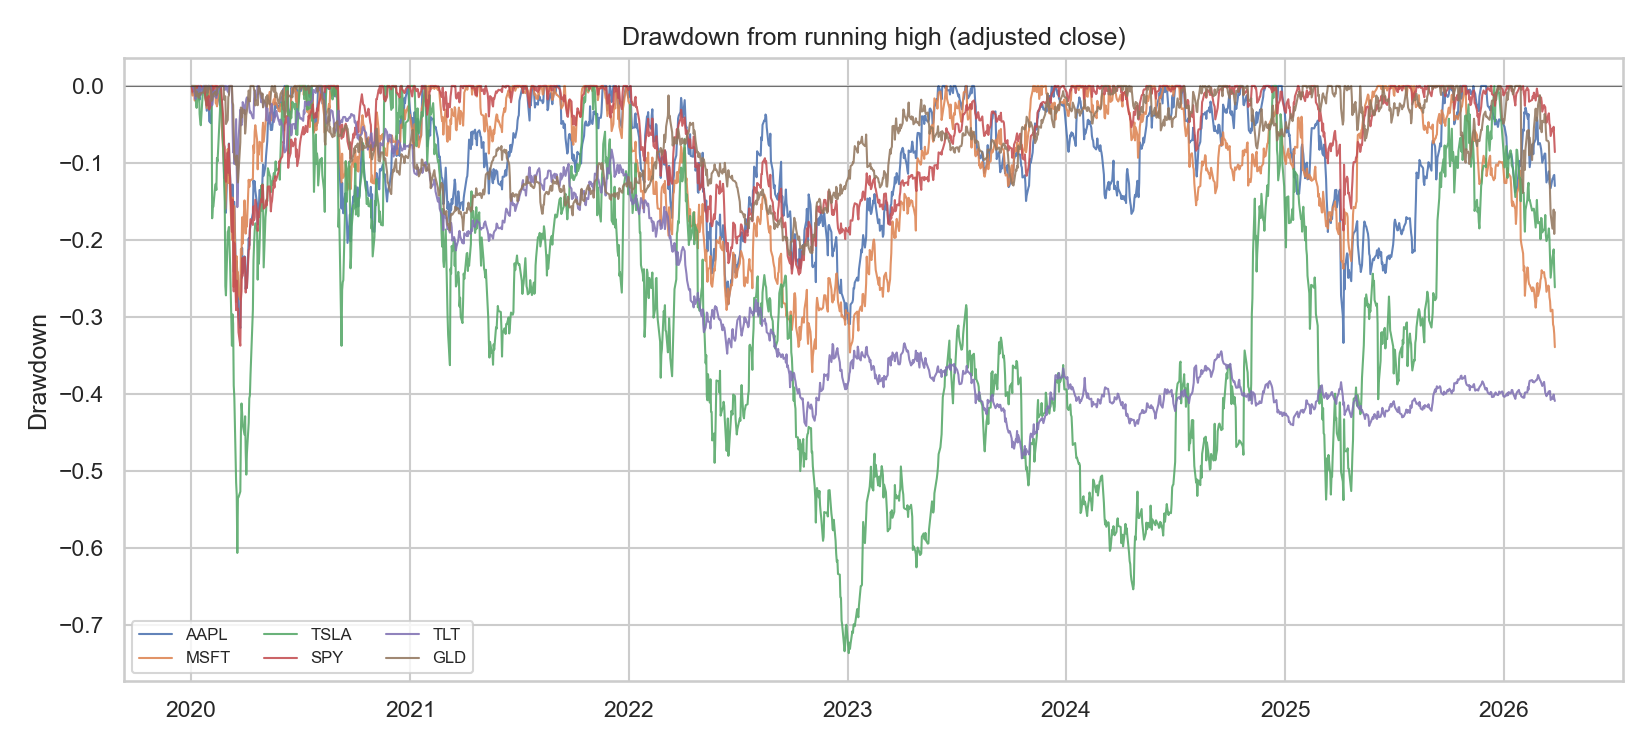
\includegraphics[width=0.95\textwidth]{data_drawdowns.png}
    \caption{Drawdown from running high on adjusted closes (processed panel). Same construction as the exploratory block in \texttt{data\_sourcing\_and\_preprocessing.ipynb}.}
    \label{fig:drawdowns}
\end{figure}

\begin{figure}[htbp]
    \centering
    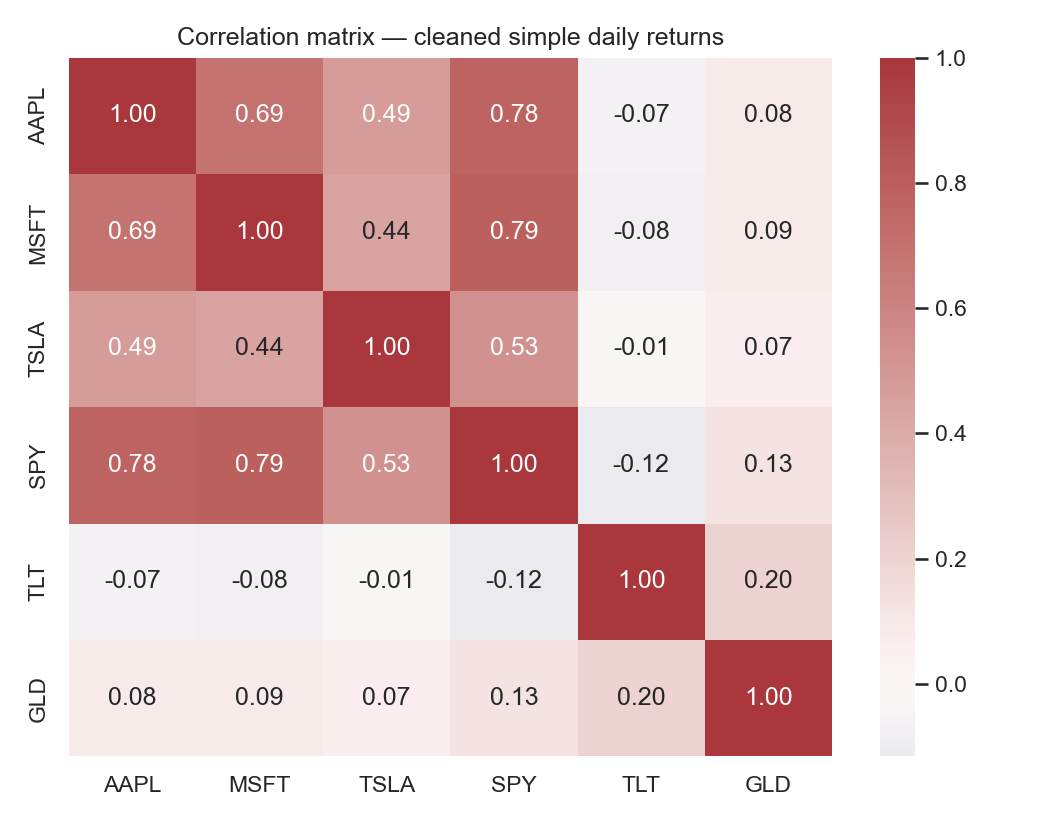
\includegraphics[width=0.72\textwidth]{data_corr_heatmap.png}
    \caption{Sample correlation matrix of cleaned simple daily returns. Regenerated from \texttt{data/processed/simple\_returns.csv} for inclusion in this report.}
    \label{fig:corr}
\end{figure}

\subsection{Cleaning rule and export}
The following extract matches the preprocessing notebook: forward-fill a \emph{bounded} number of consecutive missing observations, then drop any row that still contains a gap across tickers. Bounded imputation limits silent invention of prices; dropping incomplete rows enforces a common calendar for portfolio sums.

\begin{lstlisting}
def clean_prices(prices: pd.DataFrame, ffill_limit: int = 5) -> pd.DataFrame:
    px = prices.sort_index()
    px = px.ffill(limit=ffill_limit)
    px = px.dropna(how="any")
    return px

prices_clean = clean_prices(raw_prices)
simple_rets_clean = prices_clean.pct_change().dropna()
log_rets_clean = np.log(prices_clean).diff().dropna()
\end{lstlisting}
\begin{center}
{\footnotesize Source: \texttt{data\_sourcing\_and\_preprocessing.ipynb}.}
\end{center}

\noindent
The notebook writes \texttt{adj\_close\_prices.csv}, \texttt{simple\_returns.csv}, \texttt{log\_returns.csv}, and \texttt{dataset\_meta.json} under \path{data/processed/}. Other subsystems (offline quant, RAG tabular hooks, LSTM notebooks) can depend on those paths without re-downloading. These processed artifacts also serve as the common input layer for the return notation and risk metrics formalised in Section~\ref{sec:methodology}.

\subsection{Reproducibility}
To support reproducibility, the data preparation workflow should be run from the repository root so that file paths resolve consistently. Because Yahoo Finance data may change over time, the execution date should be recorded whenever figures are regenerated. Figures~\ref{fig:drawdowns} and~\ref{fig:corr} can be rebuilt from the processed CSVs by running \texttt{python} on \path{report/scripts/make_data_figures.py}.


\section{Methodology}
\label{sec:methodology}

\subsection{Portfolio construction and notation}
Consider $n$ risky assets. Let $r_t \in \mathbb{R}^n$ denote the vector of simple returns on trading day $t$, and let $w \in \mathbb{R}^n_{\ge 0}$ denote portfolio weights satisfying $\sum_i w_i = 1$ after normalisation. The portfolio return is
\begin{equation*}
r_{p,t} = w^\top r_t .
\end{equation*}
Vectors $w$ are supplied exclusively from the validated interface state and are not inferred by the language model, thereby avoiding implicit reweighting such as undocumented equal-weight assumptions.

\subsection{Risk and performance metrics (current build)}
The implemented pipeline computes the following quantities on the sample of portfolio and asset returns:
\begin{itemize}
    \item \textbf{Annualised volatility.} The sample standard deviation of $\{r_{p,t}\}$, multiplied by $\sqrt{252}$ under the conventional mapping from daily to annual units for equities.
    \item \textbf{Historical quantile loss.} The empirical 5th percentile of $\{r_{p,t}\}$ at a one-day horizon, reported without scaling to multi-day regulatory value-at-risk horizons; it constitutes a descriptive tail measure rather than a full loss-distribution model.
    \item \textbf{Sharpe-type ratio.} The ratio of mean daily excess return to standard deviation of daily returns, annualised by $\sqrt{252}$, with the risk-free rate set identically to zero for tractability; interpretability as a true economic Sharpe ratio therefore requires mental adjustment for the user's financing rate.
    \item \textbf{Maximum drawdown.} Computed on the compounded wealth process $\prod_s (1+r_{p,s})$ as the largest relative decline from a running maximum to a subsequent trough.
    \item \textbf{Average pairwise correlation.} The arithmetic mean of off-diagonal entries in the sample correlation matrix of asset simple returns.
    \item \textbf{Concentration (Herfindahl).} $\sum_i w_i^2$, equal to unity under perfect concentration and to $1/n$ under equal weighting.
\end{itemize}
The six scalars enter a piecewise rule-based mapping to a composite score in $[0,1]$ and to ordered risk categories (\texttt{Low}, \texttt{Medium}, \texttt{High}). Thresholds are chosen for demonstration and narrative coherence; they are not calibrated against regulatory templates.

The intent classifier vocabulary may reference additional statistics (e.g.\ Sortino ratio, beta, conditional tail expectations) that constitute planned extensions; any metric not produced by the executed code path should be explicitly identified as absent in empirical sections of this report.

\subsection{Prospective machine-learning components}
The software repository permits future integration of sequence models (e.g.\ recurrent networks for forward-looking volatility) and learned risk taxonomies. At the time of writing, categorical risk bands rely on deterministic rules rather than trained classifiers. Adoption of learning-based modules would oblige a complementary discussion of training and validation protocols, information leakage across time, and the provisional nature of forecast outputs.

\subsection{Retrieval-augmented generation}
The RAG subsystem partitions background knowledge into thematic stores (including, inter alia, ticker disambiguation aids, firm-level summaries, macroeconomic indicators, curated definitions, and strategic-allocation notes). Retrieval is conditioned on the inferred dialogue intent: only subsets of corpora are queried for a given turn. Candidate passages undergo deduplication and scoring; retrieval itself employs a hybrid of lexical matching (Okapi BM25) and dense retrieval of sentence-transformer embeddings persisted in Chroma. Logging supports retrospective measurement of retrieval quality (e.g.\ recall at fixed $k$).

In the \textbf{reference Streamlit deployment} (\texttt{chatbot.py}), assistant turns are produced solely by deterministic Python: template Markdown, numerically computed metrics, and optional retrieved excerpts concatenated in the orchestrator. There is \emph{no} second large-language-model call that rewrites the full answer in that path; richer ``answer models'' may exist in ancillary scripts or future revisions, but they are not required for the live loop described here. Relative to unconstrained generation, retrieved spans narrow---without eliminating---hallucination risk by anchoring visible text to locally stored evidence, subject to corpus coverage and chunk boundaries.

\subsection{Agent and intent orchestration}
Each utterance receives a primary intent label from Gemini among holistic portfolio analysis, single-metric interrogation, conceptual explanation, trend or outlook questioning, conversational follow-up, and general dialogue. Optional secondary intents and normalised entity fields (metrics, concepts) may accompany the classification.

Dispatch logic implemented in Python branches on the primary label. Computationally intensive paths reuse a single price fetch and return construction step where feasible; explanatory paths may issue retrieval calls with intent tags recognised by the RAG layer (\texttt{full\_analysis}, \texttt{concept\_explanation}, \texttt{trend\_prediction}). Follow-up handling surfaces the preceding assistant message from session history rather than maintaining long-horizon episodic memory. Separation of probabilistic classification from deterministic numerical execution is intentional: portfolio arithmetic remains auditable code, not prompt-dependent improvisation.


\section{System design and implementation}
\label{sec:system}

\subsection{Architecture overview}
The portfolio risk analyst is structured as a hybrid between an autonomous agent and a set of fixed agentic workflows. At the top level, it behaves as an agent. It receives a user query, classifies the intent, and selects a workflow to execute. Once an intent is identified, however, the system follows a predefined sequence of function calls rather than granting the LLM full autonomy over tool selection.

This design was deliberate. Because if we were to use a fully autonomous agent, decisions would rely on the LLM to determine which tools to invoke at each step, introducing variability in the depth and consistency of the analysis. In a system with well-defined computation dependencies (e.g., the covariance matrix must be computed before portfolio volatility, risk contribution, and average pairwise correlation can be derived), an LLM that skips or reorders steps can cause silent downstream failures. Fixed workflows guarantee that every relevant module executes in the correct order, ensuring the LLM always receives a complete picture before generating its response. This sacrifices some flexibility: a fully autonomous agent could blend intents more fluidly or adapt to unforeseen queries without rigid routing. However, given a known set of intents and a deterministic computation pipeline, the gains in reliability, debuggability, and testability outweigh the loss of adaptiveness.


\begin{figure}[H]
    \centering
    \fbox{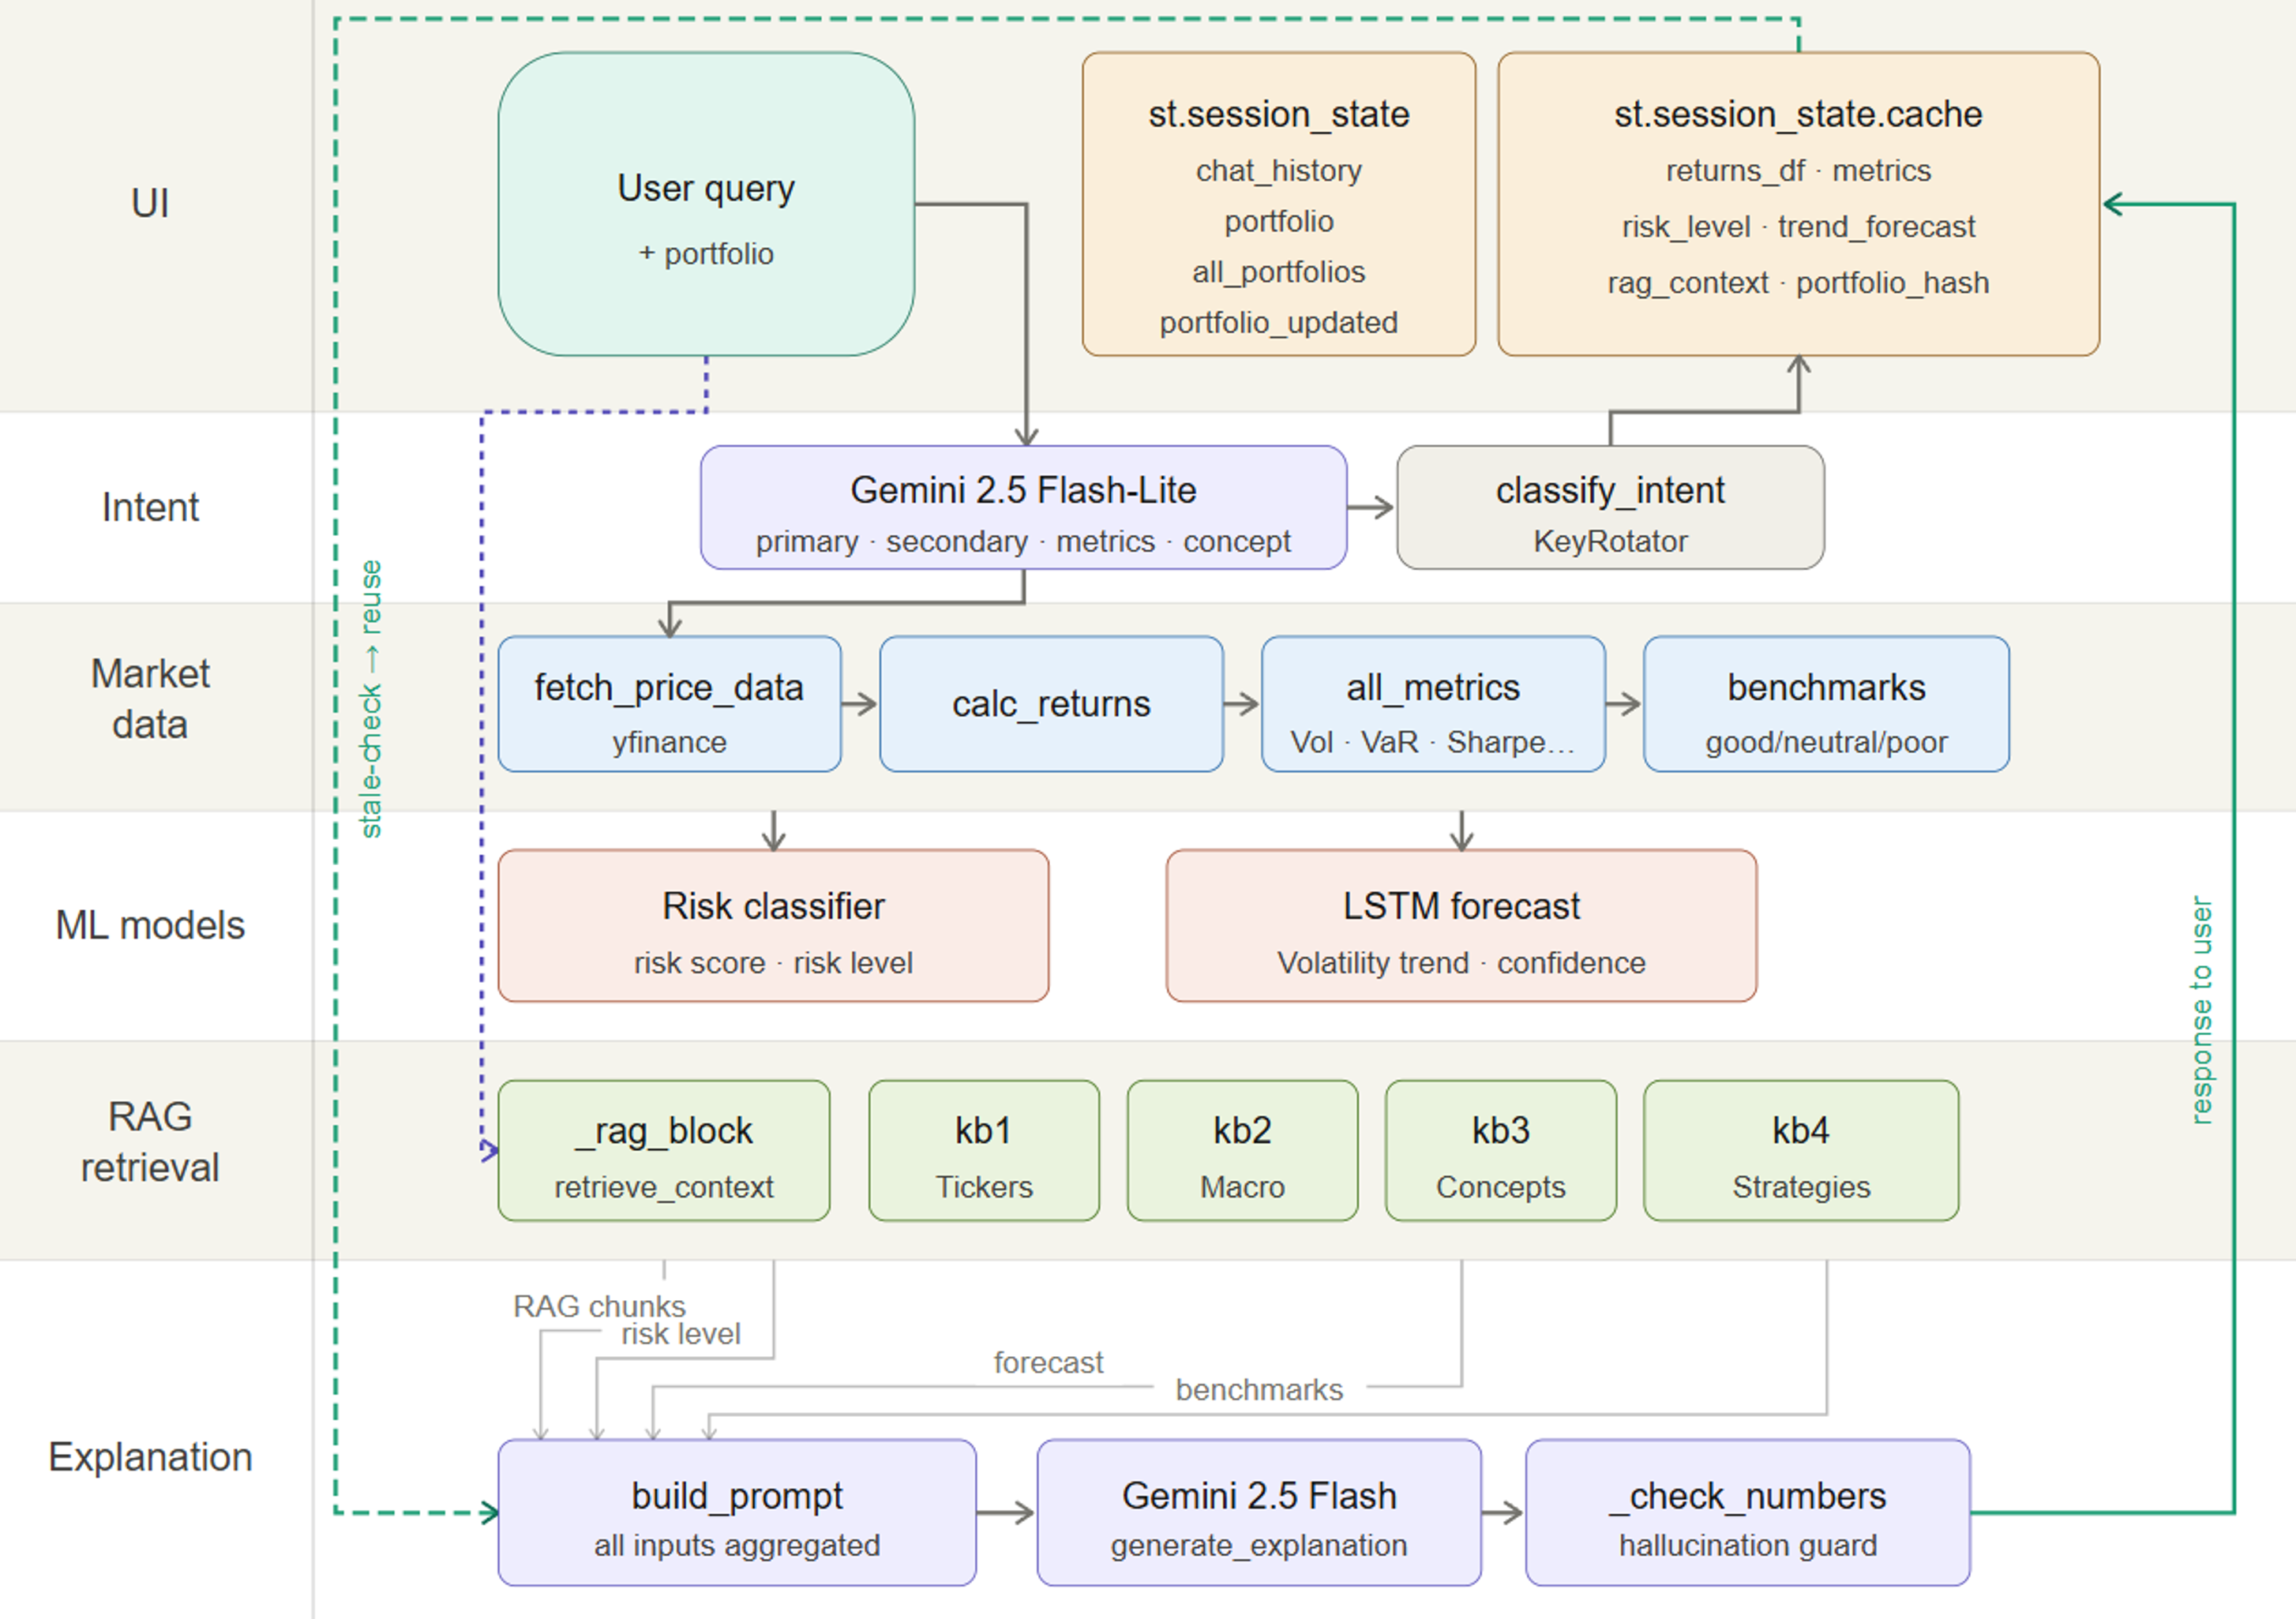
\includegraphics[width=0.75\textwidth]{archi_overview_diagram.png}}
    \caption{Diagram illustration of the overall chatbot architecture.}
    \label{fig:archi_overview}
\end{figure}

As shown in Figure~\ref{fig:archi_overview}, the system is organised into several key layers. At the \textbf{UI layer}, the user submits a query along with their portfolio via a Streamlit interface. The \textbf{intent layer} classifies the message into one of six intents (full analysis, specific metric, concept explanation, trend prediction, follow-up, or general chat) and extracts any referenced metrics or concepts required downstream.

Once classified, intents are routed through a \textbf{shared computation pipeline} managed by a backend orchestrator function, \texttt{route\_and\_execute}, which computes the information required for each intent and updates the cache accordingly. If the relevant data has already been computed and the portfolio has not changed, it is retrieved from cache to avoid redundant computation.

Furthermore, the pipeline comprises four main components:

\begin{itemize}
    \item A \textbf{data layer} that validates input tickers and extracts the price and return data required by the other components.
    
    \item A \textbf{quant component} that produces 12 risk metrics — including portfolio volatility, VaR, Sharpe ratio, beta, and skewness — from a covariance matrix computed once and reused downstream.
    
    \item An \textbf{ML component} consisting of a logic-based risk classifier (outputting a Low/Medium/High label) and an LSTM model (forecasting volatility trends with a confidence score).
    
    \item A \textbf{RAG layer} that takes the user query and portfolio tickers as input and searches across four specialised knowledge bases: Tickers, Macro, Concepts, and Strategies.
\end{itemize}

These components, and the workflow functions are detailed in the sections below.

Finally, all outputs converge at the \textbf{explanation layer}, where a \texttt{build\_prompt} function aggregates the risk metrics (tagged with their benchmark labels), RAG chunks, the risk classification, and the LSTM forecast into a single prompt for the LLM, which generates the user-facing explanation. A post-generation hallucination guard (\texttt{\_check\_numbers}) then validates that any numerical claims are consistent with the computed metrics before the response is returned.


\subsection{User interface}

The user interface for this application was developed using Streamlit, a Python-based framework that enables rapid development of interactive web applications. The interface is designed to provide a simple and structured workflow, guiding users from portfolio input to interactive analysis through a chatbot. Emphasis was placed on clarity, responsiveness, and ensuring that users provide valid inputs before accessing analytical features.

\begin{figure}[H]
    \centering
    \fbox{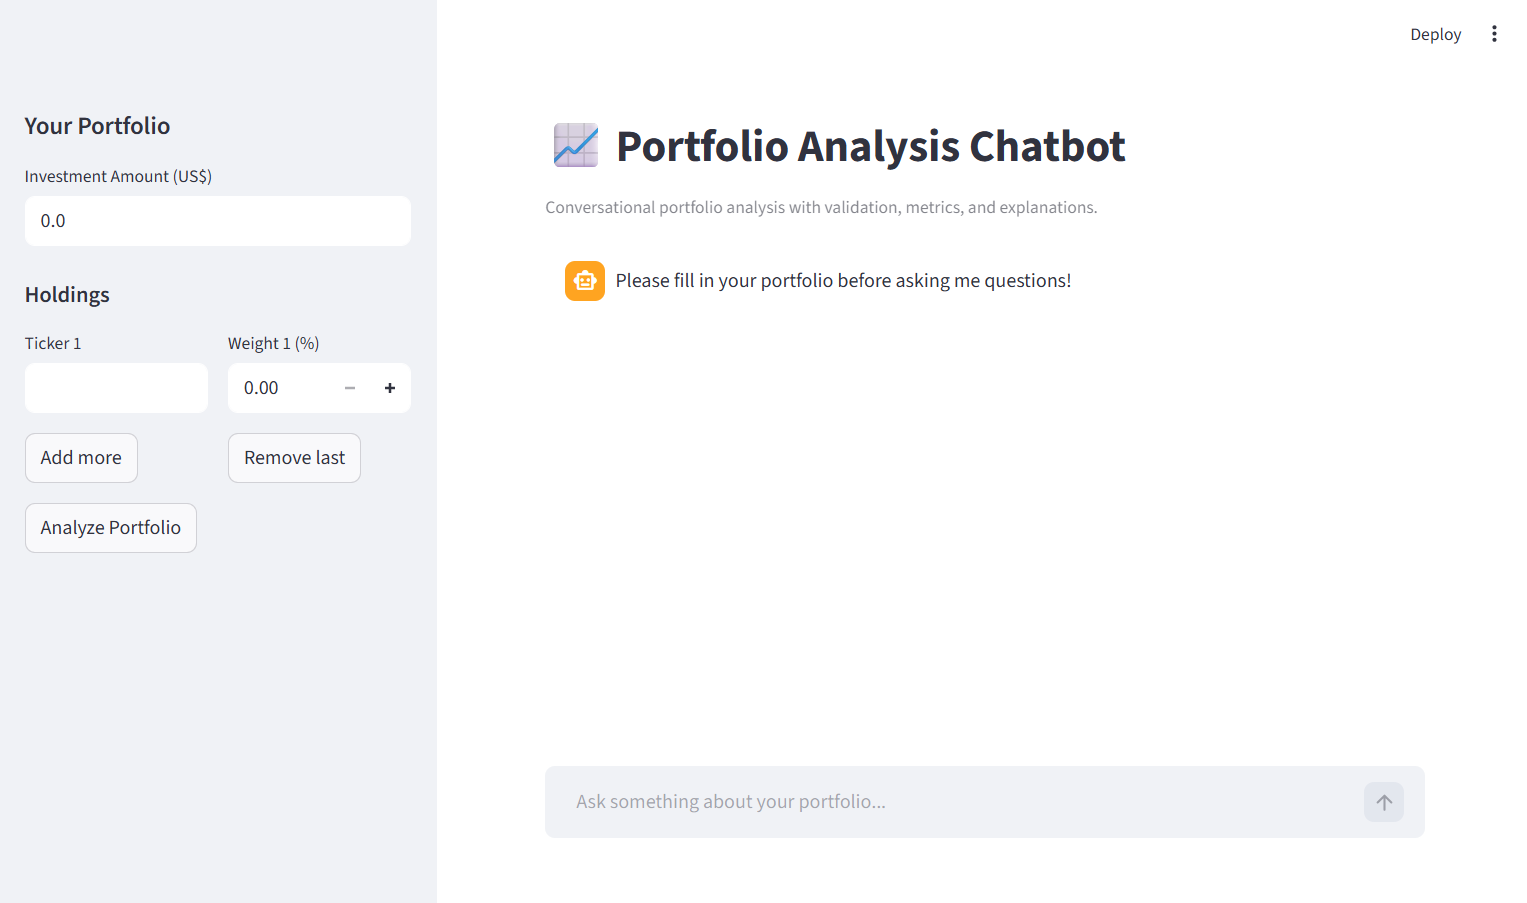
\includegraphics[width=0.75\textwidth]{ui_start_screen.png}}
    \caption{Initial interface of the portfolio analysis chatbot.}
    \label{fig:ui_start}
\end{figure}

As shown in Figure~\ref{fig:ui_start} the sidebar, located on the left, serves as the primary input interface for portfolio construction. Users are required to input portfolio components, including asset tickers, corresponding weights, and the total investment amount. Input validation mechanisms are implemented to ensure data integrity, such as verifying that portfolio weights sum to 100\% and that the entered tickers are valid. Where invalid inputs are detected, appropriate error messages are displayed, while successful validation triggers a confirmation message indicating that the portfolio is ready for analysis. In addition, tickers entered without capitalisation are automatically standardised to uppercase before being stored in the session state. The number of input fields shown in the sidebar is also managed dynamically based on the number of stocks selected by the user. This structured input process ensures that all subsequent computations are based on valid and consistent data.

The main interface consists of a chat-based interaction system that enables users to query and analyse their portfolio. Messages are displayed in a conversational format, with clear visual distinction between user inputs and system-generated responses, as shown in Figure~\ref{fig:ui_query}. below. To improve user experience, a loading indicator is shown while backend processing is underway, providing feedback that the query is being handled.

\begin{figure}[H]
    \centering
    \fbox{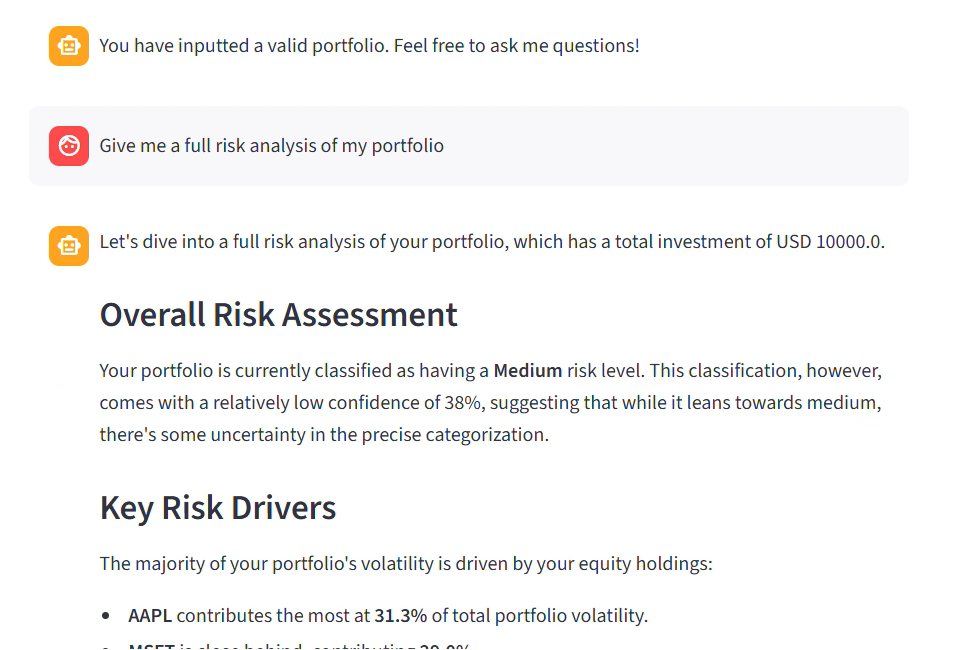
\includegraphics[width=0.75\textwidth]{ui_query_and_response.png}}
    \caption{Chat-based query and response interface of the portfolio analysis chatbot.}
    \label{fig:ui_query}
\end{figure}

A key design feature is the implementation of a chat-locking mechanism. The chat functionality remains disabled until a valid portfolio has been successfully submitted. This prevents invalid or premature queries and enforces a logical interaction flow. Once the portfolio is validated, the chat is unlocked and users are notified that they may begin interacting with the system.

To support dynamic interaction, session state management is implemented using Streamlit's \texttt{st.session\_state} functionality. This enables the application to retain key information across reruns within the same user session, including the current portfolio data, submitted portfolio versions, validation status, chat history, and portfolio-related system messages. Variables such as \texttt{portfolio\_ready} are used to control whether the chatbot is accessible, while separate storage of \texttt{chat\_history} and \texttt{portfolio\_messages} helps maintain a clean and organised interface. Additional state variables, such as the number of stocks selected and whether the portfolio has been updated, allow the interface to respond dynamically to user actions. This ensures continuity of interaction and prevents the loss of important data during use.

From a user experience perspective, the interface is designed to be intuitive and guided. Users receive immediate feedback on their inputs, are prevented from making invalid queries, and can clearly follow the progression from portfolio input to analysis. Visual cues, such as confirmation messages and loading indicators, further enhance usability and provide transparency during system processing. Overall, the design promotes a structured and user-friendly interaction, ensuring that users can efficiently navigate the application and obtain meaningful insights from their portfolio.




\subsection{Key modules}
\todo{\texttt{agent\_tools/data\_tools}, quant (if separate), \texttt{RAG/}, \texttt{workflow\_tools} (classifier, orchestrator).}

\subsubsection{Data Tools}
\subsubsection{Main Workflow Tools}
\subsubsection{Quant Tools}
\subsubsection{LSTM Tools}
\subsubsection{RAG Tools}


\subsection{Failure modes and safeguards}
\todo{Missing tickers, short history, SPY fetch failure, model/RAG errors, graceful fallbacks.}


\section{Evaluation}
\label{sec:evaluation}

\subsection{LSTM Evaluation}

\begin{table}[h]
    \centering
    \begin{tabular}{|l|c|}
        \hline
        Volatility Prediction Evaluation MSE & 0.0026 \\
        \hline
        Volatility Prediction Evaluation MAE &  0.0389 \\
        \hline
        Direction Prediction Evaluation AUC & 0.5358 \\
        \hline
        Direction Prediction Evaluation Accuracy & 0.67 \\
        \hline
    \end{tabular}

    \caption{Prediction results of volatility and future direction of portfolio on test dataset}
    \label{tab:lstm_prediction_results}
\end{table}

As seen from Table~\ref{tab:lstm_prediction_results}, the model has relatively strong accuracy in predicting future volatility of portfolio over the next 10 days, with a test MSE of 0.0026 and MAE of 0.0389. These results suggest that the model is able to effectively learn and estimate short-term portfolio risk. This result is consistent with expectations, as volatility exhibits temporal clustering, making it more predictable from historical data. Comparatively, the model struggled in predicting future direction. The low AUC of only about 0.5358 suggests that the model’s ability to distinguish between future upward and downward movements of the portfolio is only marginally better than random guessing. 

\begin{table}[h]
    \centering
    \begin{tabular}{|l|c|c|}
        \hline
          & Future Upward direction & Future Downward direction \\
        \hline
        Precision & 0.81 & 0.64 \\
        \hline
        Recall & 0.34 & 0.94 \\
        \hline
        F1-score & 0.48 & 0.76 \\
        \hline
    \end{tabular}

    \caption{Classification report of future direction of portfolio on test dataset}
    \label{tab:lstm_classification_report}
\end{table}

\begin{figure}[H]
    \centering
    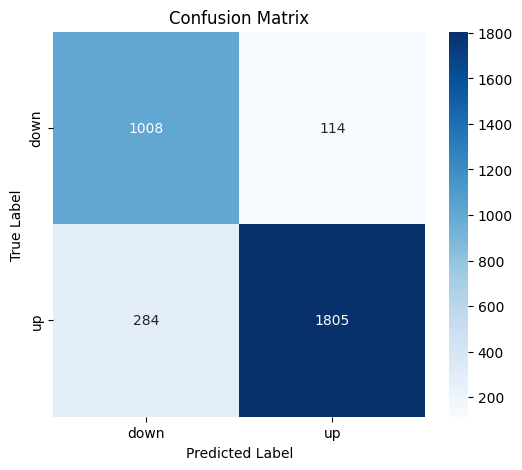
\includegraphics[width=0.65\textwidth]{LSTM_confusion_matrix.png}
    \caption{Confusion matrix on future direction of portfolio on test dataset.}
    \label{fig:lstm_confusion_matrix}
\end{figure}

As observed from the confusion matrix in Figure~\ref{fig:lstm_confusion_matrix}, the model performs better in predicting future portfolio downward movements. From Table~\ref{tab:lstm_classification_report}, the model is observed to have very high recall for downward movements, showing that it is able to identify most future downward portfolio directions. However, it has low recall for future upward movements and many future upward trends are misclassified as downward. The model struggles to learn a robust directional signal and the input feature of 60 days log-return does not contain sufficient predictive information for future direction. 

The discrepancy between volatility and direction prediction performance highlights the challenges in financial time series modeling. Volatility is generally easier to predict due to its relatively stable statistical properties like clustering, which allows the model to effectively learn temporal dependencies. Comparatively, future portfolio direction is inherently noisy and less predictable, especially when using relatively short input windows such as 60 days of log returns.

The model is also observed to be more conservative when predicting upward movements as seen from the significantly lower recall for upwards prediction. There are fewer false positives as seen from the higher precision for upwards prediction and the model is more sensitive in predicting downward movements with fewer missed negatives from the higher recall, which is relatively more desirable than the converse in a risk management context.

Therefore, while the LSTM is effective for volatility forecasting, it is less suitable for directional prediction as it struggles to extract meaningful signals for direction due to the high level of noise and weak predictability in short-term portfolio direction. 

\subsection{RAG Retrieval Evaluation}
\begin{figure}[H]
    \centering
    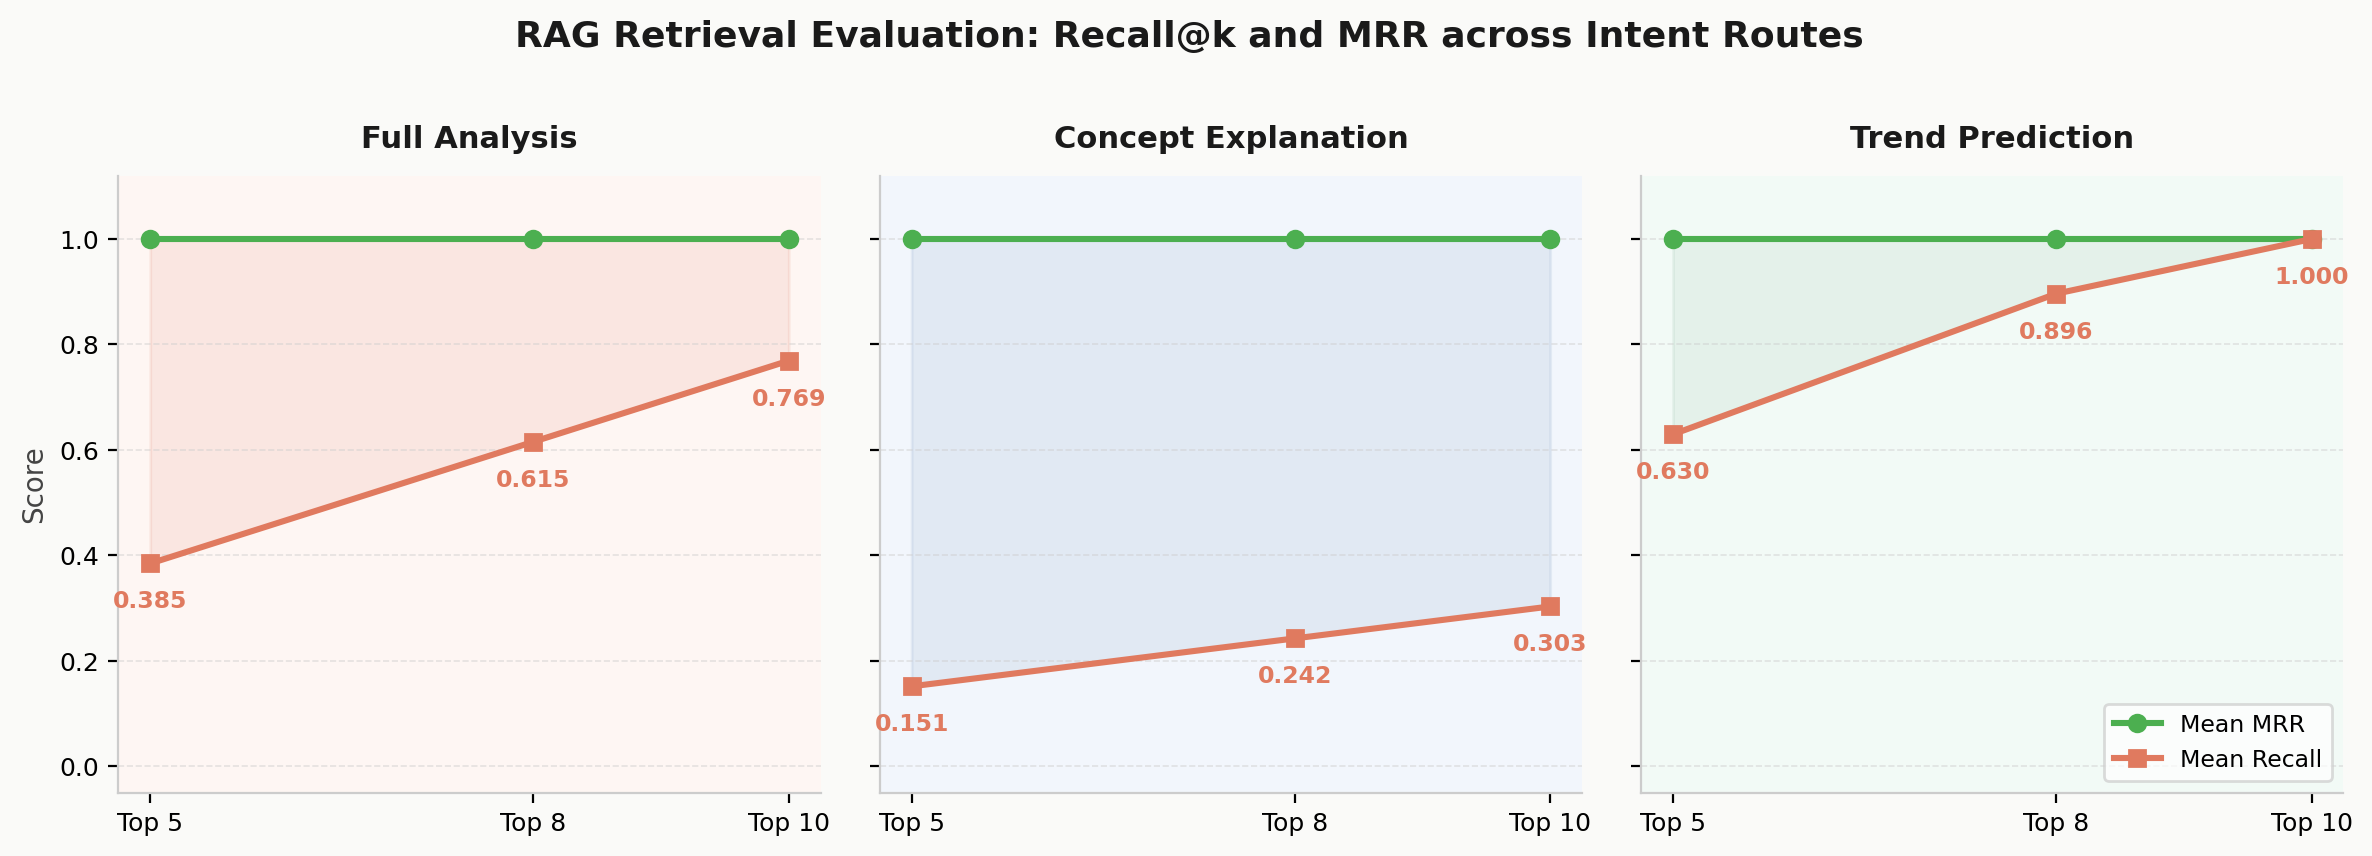
\includegraphics[width=0.75\textwidth]{rag_eval.png}
    \caption{Recall and MRR at $k \in \{5, 8, 10\}$ across three intent routes.}
    \label{fig:rag_recall_mrr}
\end{figure}

To evaluate retrieval quality, nine queries were designed spanning all four intent routes -  \texttt{full\_analysis}, \texttt{concept\_explanation}, \texttt{trend\_prediction} and \texttt{no\_intent}, at three difficulty levels: Easy, Medium and Hard. Retrieval performance was assessed using Recall@$k$ and Mean Reciprocal Rank (MRR) at $k \in \{5, 8, 10\}$. While MRR measures the rank position of the first relevant result, Recall@$k$ measures how many relevant chunks are surfaced within the top k; the two metrics are therefore complementary, a system can rank its first retrieved chunk perfectly (MRR = 1.0) while still missing out other relevant material (Recall $<$ 1.0).

As shown in Figure~\ref{fig:rag_recall_mrr}, MRR equals 1.0 across every intent at every value of k, indicating that whenever a relevant chunk is retrieved, it is consistently ranked first. This confirms that the hybrid retrieval strategy produces well-ordered results.

For \texttt{full\_analysis} queries, Recall@$k$ rises from 0.385 at k=5 to 0.769 at k = 10, reflecting consistent retrieval from a well-populated knowledge store. \texttt{Trend\_prediction} achieves the strongest recall trajectory, reaching near-perfect scores at k=10, suggesting that dense semantic search handles indirectly phrased forward-looking queries effectively.

\texttt{Concept\_explanation} records the lowest Recall@$k$ values; however, this is an artefact of knowledge base construction rather than retrieval failure. Only one relevant chunk exists per concept in the concept store, placing a hard ceiling on the system and motivating future work to expand the concept corpus.

Across all intents, increasing k consistently improves Recall, confirming that the relevant chunks exist in the index and that broader retrieval windows surface them reliably. Overall, the results suggest that the pipeline is well-calibrated for ranking quality, with the primary path to improvement lying in expanding the concept knowledge store rather than in changes to the retrieval mechanism itself.



\subsection{LLM Evaluation}
% to add

\section{Discussion}
\label{sec:discussion}

This section reflects on the system from four complementary perspectives: implementation strengths, practical weaknesses, broader limitations, and responsible use. The discussion focuses on how these considerations arise from the actual design choices described in the preceding sections.

\subsection{Strengths}

\subsubsection{Data Preprocessing}
The preprocessing pipeline is a strength because it enforces a consistent data contract before downstream analytics run. Adjusted closes reduce split and dividend artefacts, bounded forward fill plus row dropping preserve an aligned trading calendar, and automatic \texttt{SPY} insertion and ticker normalisation improve robustness for benchmark-dependent metrics.

\subsubsection{Architecture}
The key architectural strength is the explicit separation between intent resolution and deterministic execution. Intent is inferred by the classifier, but execution order is enforced in \texttt{route\_and\_execute()} through fixed intent-to-tool membership sets, rather than unconstrained LLM planning. This guarantees dependency order for metric computation (for example, covariance before derived portfolio statistics), improving reliability and debuggability. A session-level cache keyed by a portfolio hash avoids redundant recomputation when holdings are unchanged. The numeric hallucination guard further provides defence in depth: authorised numeric values are injected into the prompt and post-generation regex checks flag numbers not matching computed results. The design is also cost-aware: \texttt{gemini-2.5-flash-lite} is used for frequent structured classification, while a more capable model is reserved for explanation generation.

\subsubsection{Quantitative Risk Module}
The quantitative module computes 12 risk metrics spanning multiple dimensions of risk exposure (volatility, tail loss proxy, drawdown, risk-adjusted return, concentration, correlation, and related diagnostics). A covariance matrix is computed once and reused across dependent metrics, reducing duplication and ensuring consistency. Metrics are paired with benchmark labels so explanations remain interpretable instead of presenting isolated raw values.

\subsubsection{LSTM Forecasting Module}
The LSTM component shows strong test performance for volatility prediction (MSE \(\approx 0.0026\)). Its directional behaviour is asymmetric in a risk-appropriate way: higher precision on upward signals and higher recall on downward signals, which is desirable when missed downside warnings are costlier than false alarms. Weighted cross-entropy during training also reduces bias toward majority directional classes.

\subsubsection{RAG Retrieval Module}
The RAG pipeline achieves strong retrieval ordering performance (MRR \(=1.0\) across evaluated intents), indicating that relevant chunks are consistently ranked at the top when available. Hybrid retrieval (dense + lexical with reciprocal rank fusion) and intent-conditioned routing improve precision by restricting search to relevant stores. For trend-style intents, high Recall@\(k\) at larger \(k\) suggests the semantic channel can still surface useful context for less direct forward-looking queries.

\subsubsection{User Interface}
The interface enforces a guided flow through ticker/weight validation, automatic ticker normalisation, and chat-locking before a valid portfolio is submitted. These checks reduce malformed requests reaching backend tools. Immediate feedback messages and loading cues increase transparency during processing and improve usability.



\subsection{Weaknesses}

\subsubsection{Data Preprocessing}
A practical weakness is reliance on vendor-managed historical data: Yahoo Finance may revise adjusted price histories over time, so regenerated datasets can differ across runs even when the code is unchanged. In addition, the quantitative pipeline uses simple returns whereas the LSTM pipeline uses log returns. Although this choice is defensible, it reduces cross-module transparency and makes direct comparison less intuitive.

\subsubsection{RAG Retrieval Model}
The RAG pipeline relies on a relevance threshold. When no chunk passes threshold, fallback top-\(k\) context may still be passed to generation, increasing risk of weak grounding. Embedding freshness is another fragility: if stores are updated while refresh is deferred, retrieval can lag current content. Operationally, vector-store persistence errors can also interrupt retrieval without rich user-facing recovery. Finally, uneven store population (for example, sparse concept chunks) can cap attainable Recall@\(k\) irrespective of retriever quality.

\subsubsection{User Interface}
Reasoning visibility remains mostly backend-facing; users do not see intermediate tool calls or retrieval traces unless additional surfacing is implemented. Session state is memory-backed and reset on refresh, so chat and portfolio continuity are not persisted across browser sessions. The strict chat-locking policy is safe but rigid for exploratory users who may want non-portfolio explanatory queries before full submission.

\subsubsection{Explanation Layer}
The hallucination guard currently flags suspicious numbers but does not automatically suppress or regenerate responses, so remediation is incomplete. Conversation context is truncated to a short recent window, which may degrade coherence for long sessions. Ambiguous multi-intent queries can also lose secondary intent when classifier confidence is low, resulting in incomplete context assembly for generation.



\subsection{Limitations}

\subsubsection{Data Preprocessing}
The preprocessing layer is also limited by its data source and scope. Dependence on \texttt{yfinance}/Yahoo Finance creates a single external point of failure, while the use of end-of-day adjusted closes excludes intraday dynamics, bid-ask effects, and liquidity stress. The default window beginning at \texttt{2020-01-01} captures recent regimes but not longer historical cycles, and survivorship effects are not explicitly modelled.

\subsubsection{Architecture}
The system is scoped to long-only portfolios and excludes options, leverage, and short positions. Instrument coverage is constrained by vendor availability. Historical-metric interpretation implicitly assumes a stable holding period over the sampled window, which may not match recently constructed portfolios. Conversation and comparison memory are also bounded by design.

\subsubsection{LSTM Forecasting Module}
The LSTM is stronger on volatility magnitude than directional forecasting under noisy short-horizon returns. Training data are largely synthetic portfolio constructions, which may not fully capture real deployment distributions. Macro signals (rates, regime indicators, event features) are not explicit model inputs, limiting robustness to abrupt regime shifts.

\subsubsection{RAG Retrieval Model}
The embedding model is general-purpose rather than finance-tuned, so domain-specific terminology may be underrepresented in vector space. A cross-encoder reranker is not currently in the retrieval stack.


\subsubsection{Explanation Layer}
Both Gemini models used are general-purpose, not financial-domain-specialised. Multi-intent handling exists but depends on secondary-intent emission quality, which can fail silently under ambiguous phrasing.


\subsection{Ethics and responsible use}
This system is a research prototype and does not provide regulated financial advice. Outputs should therefore be interpreted alongside professional judgement rather than treated as standalone recommendations. While retrieved citations and numeric grounding checks improve transparency, they do not eliminate model risk or guarantee factual correctness under all conditions. Reported values are historical-statistical descriptors under explicit assumptions, not forward-looking guarantees.


\section{Conclusion}
\label{sec:conclusion}

\todo{Summarise achievements, main takeaway for a portfolio risk assistant, and concrete future work (e.g.\ live data, more metrics, user study).}


\subsection{Key Outcomes}

\subsection{Possible Future Improvements}


\subsubsection{Architectural Level}


\subsubsection{LSTM Component}


\subsubsection{RAG Pipeline}

\subsubsection{LLM Agent}

\subsubsection{User Interface}

\subsection{Conclusion}


\bibliographystyle{plainnat}
\bibliography{references}

\end{document}
